\documentclass[11pt]{article}
\usepackage[authoryear]{natbib}
\usepackage{amssymb}
\usepackage{graphicx,epsf}
\usepackage{bibspacing}
\oddsidemargin 0.0in
\evensidemargin 0.0in
\topmargin -0.3in
\textwidth 6.2in
\textheight 8.8in

\def\farcs{\hbox{$.\!\!^{\prime\prime}$}}  % Fractions of arcseconds
\def\arcsec{\hbox{$^{\prime\prime}$}}
\def\apj{ApJ}  
\def\apjl{ApJL}  
\def\aap{A\&A}  
\def\aj{AJ}  
\def\mnras{MNRAS}  
%\def\nat{Nature}  

\begin{document}

\title{RADLite manual (version 1.1)}
\author{Klaus M. Pontoppidan (pontoppi@gps.caltech.edu)}

\maketitle

\section{RADLite philosophy}

Welcome to RADLite. RADLite is a raytracer optimized for rendering large numbers of lines for dusty axisymmetric (2D) structures over, in principle, the entire
thermal wavelength range UV-millimeter.  It is {\it not} a stand-alone code, as it requires the input of an axisymmetric dust temperature structure. 
Rather, it is designed to take advantage of the general availability of dust radiative transfer codes, and does not attempt to re-invent the wheel. 
Currently, RADLite is a fully functional backend to the well-tested and much used dust code RADMC by C. P. Dullemond. However, any axisymmetric 
dust code can provide input to RADLite, although doing so will probably require that a simple interface is developed in order to produce a dust temperature and scattering source function input array in the correct format. I imagine that RADMC will serve the needs of nearly every RADLite user, in particular since it is a freely available code. 

RADLite is essentially a highly stripped-down version of the very general code RADICAL \citep{Dullemond00}, but with certain fundamental
additions that aid in the speedy rendering of line spectra and images. RADICAL itself also spawned the code RAYTRACE, which produces
continuum SEDs and images with input from RADMC. In this way, RADLite can be thought of as a sister code to RAYTRACE, only more general, since it
also includes lines.  

\subsection{When to use RADLite?}

There are at least two distinct approaches when it comes to modeling line observations in astrophysics, in particular molecular
line modeling: 1) Some like to understand chemistry and line/dust excitation processes on a fundamental level and may develop
highly advanced and elaborate models that attempt to predict properties of various astrophysical objects -- for instance, protoplanetary disks. 
Because they are so elaborate, such codes tend to be very specialized for a specific geometry or set of parameters, and may be difficult and cumbersome to 
use for someone who just wants to interpret their set of observations. 2) Others, usually more observationally based, want to place their
data into a relative context, perhaps by deriving gas temperatures, determine average abundances, etc of a sample. Such studies may be critized for being over-simplified, 
for instance, not taking into account complex geometries when deriving basic parameters from unresolved spectra. RADLite is a code that may be 
used to bridge those two approaches. Given a chemical code, RADLite will be able to rapidly render spectra that can be used to predict observations. 
Conversely, given data, RADLite is fast enough that it can be used to search a parameter space to fit abundances and abundance structures that in turn
can be used to test chemical models. 

\subsection{RADLite in the infrared}

There are other codes that accomplish similar tasks as RADLite, but these are generally optimized for use with submillimeter/millimeter molecular lines. 
One example is SKY (as part of RATRAN) by Michiel Hogerheijde and Floris van der Tak. RADLite, on the other hand, was developed for use in the infrared, 
and therefore includes are more complete treatment of dust absorption/emission and scattering. It also takes explicit steps to deal with a very wide
range in velocity space in a stable way. For instance, for protoplanetary disks in the infrared, one may have emission components that are 100 km/s wide, 
but with absorption components that are <1 km/s wide. Since radiative transfer is generally a highly non-local problem, this can cause 
problems in codes that do not explicitly try to deal with gridding issues in structures with large velocity gradients. More details
on what this means can be found in \cite{Pontoppidan09}, and there is no reason to repeat it here. Finally, the infrared spectra of, in particular, 
molecules are very rich. Water has 1000s of strong lines in the 3-200\,$\mu$m region. RADLite is designed to be able to efficiently render that many lines and
to construct the resulting line+dust spectra. 

\subsection{Line excitation}

RADLite is not an excitation code. It is a raytracer, so will need input level populations to run. It is straight forward to set level populations
to LTE, using either the dust temperature from RADMC, or an input gas temperature. This can be done using the built-in RADLite setup script. If the user
wishes to calculate the detailed balance level populations, this will have to be supplied by an external excitation code in a single file with a specific format.
I envision that use can be made of the various existing excitation codes by the development of various interfaces. Thus far, we have an interface
to the the excitation code beta3D as described in \cite{Meijerink09}. This is an aspect that we are actively working on, so stay tuned. For now, RADLite is a most
effective tool for thermalized lines. 

\subsection{Caveat emptor}

As these things tend to be, RADLite is developed on borrowed time. So while I try to make it as stable and
user friendly as possible, I expect most users to run into some problems getting it to run properly. I have
only tested the code for a small range of applications and platforms. There are 
a number of known bugs, usually the kind that causes the code to crash, not the kind
that produces wrong results -- the code is so far passes the benchmark tests
that I have been able to do \citep[more details in ][]{Pontoppidan09}. 

\section{Installation}

I am running RADLite on Intel Mac platforms, and I am using the Intel Fortran compiler. So I do not
yet consider the code ``portable'', because it has not been tested yet on other platforms. For a 
while, the main limitation was the non-availability of a 64-bit Gnu compiler, but since that seems to
have been solved, it should be more portable. 

\paragraph{Installation procedure:}
\begin{itemize}

\item First make sure that you have a 64 bit processor and a 64 bit Fortran compiler. You will also need
a reasonably new version of IDL (>6.0). RADLite should run fine on a 2 core Intel processor, but 4 cores are 
recommended for optimal performance. You will also need at least 2GB of memory, 8GB recommended. Finally, 
you will need the full IDL astronomy library installed to get the most out of the post-processing IDL scripts: {\tt http://idlastro.gsfc.nasa.gov/}

\item Install RADMC as instructed on the RADMC website: \\
({\tt http://www.mpia.de/homes/dullemon/radtrans/radmc/})
Note that you will only {\it need} the RADMC executable, not the setups that
come with RADMC. You could use those just fine, but RADLite comes
with some ready-to-use RADMC setups, so no need to get them mixed up! Once you are
more familiar with how everything works, you can experiment with adding your own setups. 

\item gunzip and untar the RADLite tarball in the folder of your choice:

{\tt gunzip RADLite\_XXX.tar.gz}\\
{\tt tar -xvf RADLite\_XXX.tar} \\

This should make a main folder called {\tt RADLITE\_VX.X}
\item If you have an Intel Mac, you can skip the next two compilation steps. The RADLite distribution
comes with a pre-compiled executable for Macs. 

\item Go to the Fortran RADLite folder: {\tt RADLITE\_VX.X/RADLITE/} and edit the Makefile to use the compiler you want. You will have to
uncomment the appropriate compiler line and comment the others. Right now you can choose between ifort and gfortran.  

\item Now compile RADLite by typing {\tt ./INSTALL} from the {\tt RADLITE\_VX.X/RADLITE/} folder. This should generate two executables, one
for spectroscopy, and one for imaging. 

\item RADLite currently comes with two example model setups, one for a protoplanetary disk, and one for an infalling Shu envelope.
Each has its own subfolder in the main {\tt RADLITE\_VX.X/} folder. Head to the {\tt RADLITE\_VX.X/RUN\_EXAMPLE\_PPDISK/} folder. Each model 
run folder contains two input parameter files; one for RADMC and one for RADLite. For historical reasons, the RADMC input file is called {\tt problem\_params.pro} (this
is the same for any regular RADMC run). At the end of the {\tt problem\_params.pro} file there are a number of paths that you may need to edit to match your
preferences. At a minimum, you will need to point to the Kurucz folder in the RADLite main folder if you want to include Kurucz input stellar spectra. Most users
will only need to make this change. The RADLite input parameter file is called {\tt line\_params.ini}. Open this in your editor and edit the 'main\_path' keyword to point to
your {\tt RADLITE\_VX.X} folder. 

\item Finally(!), you need to add the folder containing all the RADLite IDL scripts to your IDL path. You can do this in your .cshrc or .bashrc, depending on
your shell. My .cshrc line is: 
{\tt setenv IDL\_PATH     \$IDL\_PATH{:}+/Users/pontoppi/WORK/RADLITE\_V1.1/PRO}.
Don't forget to source the .cshrc for the change to take effect!

\item That's it! You should now be good to go. 

\end{itemize}

\section{Running the code}

\subsection{Calling Sequence}
If you are already familiar with RADMC, the way RADLite functions should be familiar. RADLite takes the place of RAYTRACE to generate spectra and images. 
The normal sequence of a model run is:

\begin{itemize}
\item You will always run the model from within the run folder. In our case, that would be {\tt RADLITE\_VX.X/RUN\_EXAMPLE\_PPDISK/}. 
Now start IDL. 

\item The RADMC setup is generated using: \\
{\tt IDL> .r problem\_setup}

\item You can now exit idl and run RADMC, or simply run it from within IDL using: \\
{\tt IDL> \$radmc}

\item Once RADMC has completed its run, you are ready to actually do something with RADLite. You should now edit the parameters in {\tt line\_params.ini} to suit your needs. 
There are a lot of parameters, and not all are really useful, a few are no longer used at all. However, the parameter file is commented, so
most things should be self-explanatory. One important technical parameter is the number of processor cores to use {\tt ncores}. Obviously, this
is system-dependent, and you do not want to use 3 cores if you only have 2! Essentially, this is a highly simplified parallelization. Modern operating systems
running on multiple-core processors will assign processes to different cores to even out the load. This means that on a 4 core system (like my own), I can
start three simultaneous RADLite processes that will automatically each run on a separate core, leaving one core free for other tasks (such as reading the news while
I wait for my run to complete). RADLite is thus made to start, say, 3 parallel processes at any one time. Each process will render {\tt subN} lines. Each 
process resulting in the rendering of {\tt subN} lines is called a subrun. The specific lines that are rendered
is determined by setting a wavelength range (using keywords {\tt min\_mu} and {\tt max\_mu}), as well as which molecule to actually render by specifying the hitran isotope code
with {\tt isot}. If the total number of lines is 98 and subN is 20, RADLite will generate 5 separate runs; 4 with 20 lines and 1 with 18. With 3 cores made available, these runs will 
take up 3 cores for the first three runs, followed by 2 cores for the final runs. 

\item RADLite is executed using: \\
{\tt IDL> .r line\_run}\\
{\tt IDL> line\_run, run\_name='my\_run'}\\

RADLite will now render lines in the specified sequence. When complete, IDL will issue a {\tt stop} statement. This allows the user to check
whether all processes are really complete (I use a top command to check on any active process). When you are sure that everything
is finished, type:\\
{\tt IDL> .c }\\

This will copy all run files into a time-stamped sub-folder in the run directory beginning with {\tt my\_run} (or whatever you specified when
you ran {\tt line\_run}. That way, you will not be overwriting previous runs. 

\end{itemize}

\subsection{Flow Chart Of Routines}

\begin{figure}
\centering
\includegraphics[scale=0.4]{RADLite.pdf}
\caption{Routines called during a non-LTE run of RADlite.  The output is given in red for each routine.}
\end{figure}

\subsection{Description of Routines}

\begin{itemize}

\item{\tt extract\_lambda.pro}\\
User inputs desired levels according to maximum vibrational and rotational level.  The levels are extracted from the molecular file as a whole, as are all transitions involving those levels.  All collisional transitions are weighted according to collisional partner abundance and interpolated onto one temperature grid, for interpolation in P.pro.

\item {\tt hitran\_extract.pro}\\
Extracts molecular information from HITRAN file and writes molecular data file.

\item {\tt lamda\_extract.pro}\\
Similar to {\tt hitran\_extract} except extracts data from LAMDA formatted file.

\item {\tt line\_run.pro}\\
Breaks run down into sub-runs according to number of lines per run and number of cores allotted.  Calls {\tt problem\_lines} to create level population information and then the RADLite executable to generate spectra.

\item{\tt nlte.pro}\\
This program solves the equations of statistical equilibrium.  First, P.pro generates all the rate coefficients for the level transitions and then uses a Newton-Rhapson iteration to converge onto a solution for the level populations.  The user can set a convergence criteria as a maximum fractional difference between iterations.  

\item{\tt nlte\_main.pro}\\
The mean intensity field is read from the RADMC output and interpolated to the desired frequencies.  Also, if the user chooses to specify the number of levels to populate (using maximum v and j values), these levels and the associated transitions are selected.  The radii are then processed separately, either consecutively or in parallel using the build\_bridges function of IDL, and nlte.pro is called for each radius.  All the radii are combined at the end and the population file levelpop\_nlte.fits is created.

\item{\tt P.pro}\\
The optical depth along the vertical column is computed and used to calculate the probability of escape (Pesc.pro) and of being captured and pumping the lines (Ppump.pro).  These probabilities, along with the interpolated intensity field, the Einstein A and B coefficients, and the collisional rate coefficients, are used to calculate the rate of transitions between any two levels.  The output is an n by n matrix where n is the number of levels specified by the user.  The final row in the matrix is populated with the total abundance in the cell in order to conserve mass and constrain the solution.

\item {\tt problem\_lines.pro}\\
Problem lines generates the gas structure input files including temperature, density, abundance, turbulence and velocity profiles, each gridded with height and radius in the disk.  The level populations of the molecule are determined and stored in the levelpop\_moldata.dat files, with the meta data stored in levelpop.info.  If non-LTE has been selected, nlte\_main.pro is called, otherwise level populations are set to LTE using the temperature structure and partition sum that was calculated previously.

\item{\tt read\_molecule\_lambda.pro}\\
This routine reads the molecular information, including energy levels and radiative and collisional transition rates, from an input file and returns an easily manipulated package.

\item {\tt write\_linespectrum\_inp}\\
Writes linespectrum.inp file.
 
\end{itemize}

\section{Inspecting the result and generating spectra}

Congratulations! When you reach this point, you have in fact rendered your first lines. However, they are at this point stored as ascii tables in
velocity space, making them hard to visualize. There is an IDL script called {\tt read\_line()}, which allows you to read a 
set of lines into an IDL structure. Note that RADLite as default generates lines for a source at a distance of $D=1$ pc.
This makes it easy to scale the fluxes to whatever distance the user wishes using $\rm Flux_{scaled} = Flux_{RADLite}/D^2$.
The lines are rendered in velocity space, and so that is what {\tt read\_line} will return. 
I recommend that you always use {\tt read\_line} to inspect the lines you have created. 

\begin{figure}
\centering
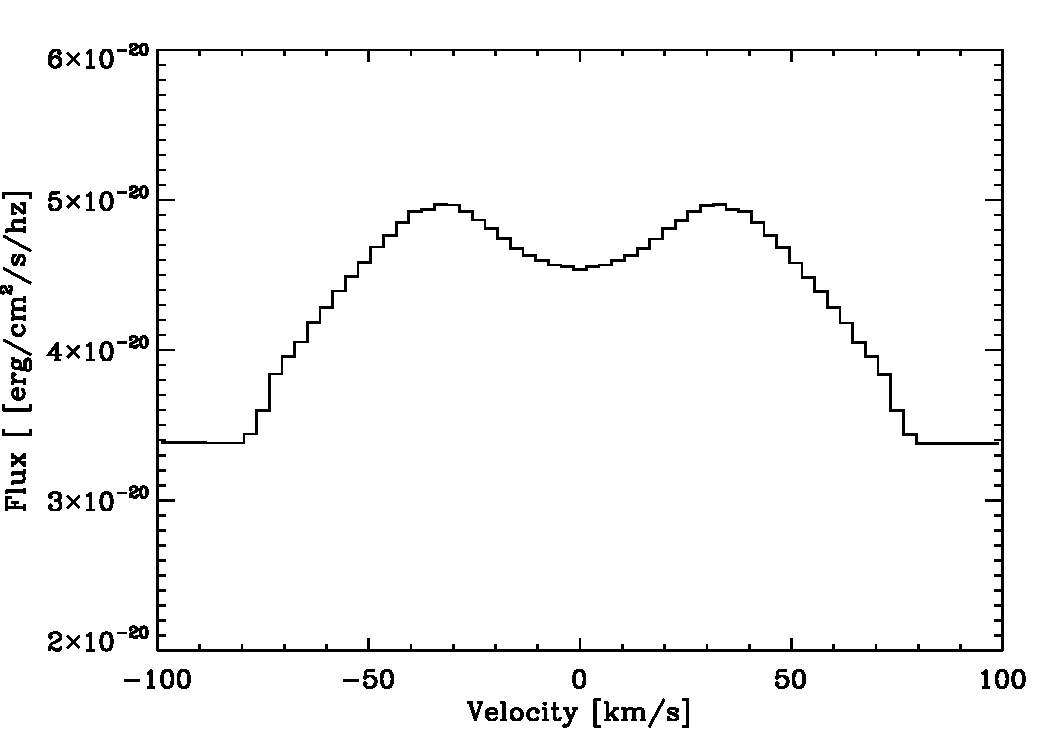
\includegraphics[width=12cm]{CO_exampleline.pdf}
\caption{CO $v=1-0$ P(7) line for the example protoplanetary disk as it appears when generated by RADlite and read by {\tt read\_line}. }
\end{figure}

However, what you probably want to do, eventually, is to generate a full spectrum that can be compared directly
to observations. To do this, you need to combine the lines. The way this is done is simple, but makes a significant assumption: Namely that lines do
not interact. In the current version of RADLite, lines are rendered separately, so very densely spaced lines may not combine correctly. Currently, 
it is up to the user to determine when this is a problem. NOTE: Lines often overlap without interacting. In protoplanetary disks, emission lines in fact rarely
interact. This only happens when the line spacing is less than the local line broadening, so for lines with rest frequencies that lie within a few km/s of eachother. 
This aspect is further discussed in \cite{Pontoppidan09}. My hope is that line overlaps can be included in the future, but for now, beware of this issue. 

Once the RADLite run is complete, you can generate a full spectrum using the idl command:\\
{\tt IDL> genspec}\\

Note that {\tt genspec} right now requires that the line spectrum is wider than $\sim$1000\,km/s, so do not try it for really narrow spectral ranges. The {\tt genspec}
tool allows for the simulation of various instrumental parameters, such as spectral resolving power and sampling, distance to the source (in parsec) and addition of noise.
It also allows a user to combine lines from several different runs, with certain restrictions, using the {\tt multiruns} keyword; this is a list of paths, e.g. {\tt multiruns=['path1','path2','path3']}.
Applications of {\tt multiruns} can be to combine isotopologues of CO, or ortho- and para-water. 

Running {\tt genspec} results in the generation of a plot (in an .eps file), as well as a .fits file containing (in a .fits extension) the full rendered spectrum (called 'model.fits'). 
The model spectrum can be read into IDL using:\\
{\tt IDL> spectrum = MRDFITS('model.fits',1)} \\
{\tt spectrum} is now an IDL structure, which we recall can be inspected in IDL using:\\
{\tt IDL> help, spectrum, /str}

\section{Imaging with RADLite}

As the spatial resolution of telescopes improve, in particular in the infrared, you may wish to figure out whether your line emission
may be extended. RADLite provides the ability to generate image cubes and combine them with a simulated telescope to predict what a 
line imaging observation may look like. In fact, the spectra are generated by internally integrating image cubes. The images are
not rendered with regularly spaced pixels, in the way that most people think of an image. Rather, the images are rendered using a 
two-dimensional circular grid with the same radial spacing as the input density grid. For instance, the RADMC grids are typically
logarithmically spaced in the radial direction because this allows for an adequate sampling both the inner and outer regions of a 
protoplanetary disk. This is good for accurately calculating lines, but is not directly translatable to a computer screen. Imagine a typical disk around
a T Tauri star with an inner radius of 0.1 AU and an outer radius of 100 AU. to properly sample the image of the inner disk, it may be necessary to
use 0.01 AU pixels (or smaller!), resulting in a total image size of $>$10,000$^2$ pixels. The vast majority of those pixels would simply oversample
the outer disk. 

Hence, RADLite is equipped with resampling scripts that can convert the so-called 'circular images' to rectangular (flux-conserved) images.
There are also tools available that can, with limitations, generate images as viewed by a telescope of a given size and instrument with a given 
sensitivity. The resampling tool is called {\tt imcir\_conv}. This IDL script will generate .fits image cubes that can be inspected
with your favorite image viewer: ds9, skycat, gaia, etc. {\tt imcir\_conv} is great for inspecting your model, and also to check if there are
sampling problems when rendering spectra; while RADLite tries to avoid some sampling pitfalls automatically, it is not failsafe, 
and still requires due diligence! 

\subsection{Running {\tt imcir\_conv}}

First you must generate a circular image cube of your line(s). This is done by running RADLite with {\tt image = 2} in line\_params.ini. The
only difference between this and the spectral rendering {\tt image = 0} is that the circular image is saved to a file called 
{\tt lineposvelcirc\_moldata\_X\_Y.dat}, where X is the subrun number and Y is the line within the subrun. For the circular images, 
a separate file is generated for each line, as opposed to a spectral run in which a single file is generated for each subrun. The reason that the
circular image files are not always saved is simply that they are quite large (20-30 Mb per line), which could be an annoying 
problem when rendering a large number of lines.  

An image can be generated by running {\tt imcir\_conv} on the relevant {\tt lineposvelcirc} file. Say, we want to generate an image cube of the inner 
$0.5\times 0.5$ AU with a sampling of 0.0005 AU and save the result in the file ``test.fits'', it can be done like this:\\

{\tt imcir\_conv, 'run\_Jan\_1\_22:34/lineposvelcirc\_moldata\_0\_1.dat',\$\\
xs=0.5, ys=0.5, nx=1000, ny=1000, saveit='test.fits'}\\

{\tt imcir\_conv} will also plot the result to a postscript file using the {\tt plotit} keyword:\\

{\tt imcir\_conv, 'run\_Jan\_1\_22:34/lineposvelcirc\_moldata\_0\_1.dat',\$\\
 xs=0.5, ys=0.5, nx=1000, ny=1000, /plotit, scale=20}\\

The -51 km/s channel intensity map as plotted by {\tt imcir\_conv} is shown in Figure \ref{imcir_ex1} (the {\tt scale} keyword is used
to change the cuts for the scaling of the image). The astute reader will notice that the line emission has 
a little ``rough'' appearance. This is due to interpolation errors from the use of a 2D interpolation scheme on a grid that
does not have a very fine ray (circular pixel) sampling ({\tt imcir\_conv} uses
IDL TRIGRID). In general, images will require a significantly finer ray sampling than pure spectra. The user is invited to experiment, but will
likely find that while a given ray sampling produces nice lines, images need a little more TLC\footnote{Tender, loving care}. You can ask
{\tt imcir\_conv} to plot the rays on the images using the {\tt plgrid} keyword. This is great for troubleshooting: \\

{\tt imcir\_conv, 'run\_Jan\_1\_22:34/lineposvelcirc\_moldata\_0\_1.dat',\$\\
xs=0.5, ys=0.5, nx=1000, ny=1000, /plotit, /plgrid}\\
 
\begin{figure}
\centering
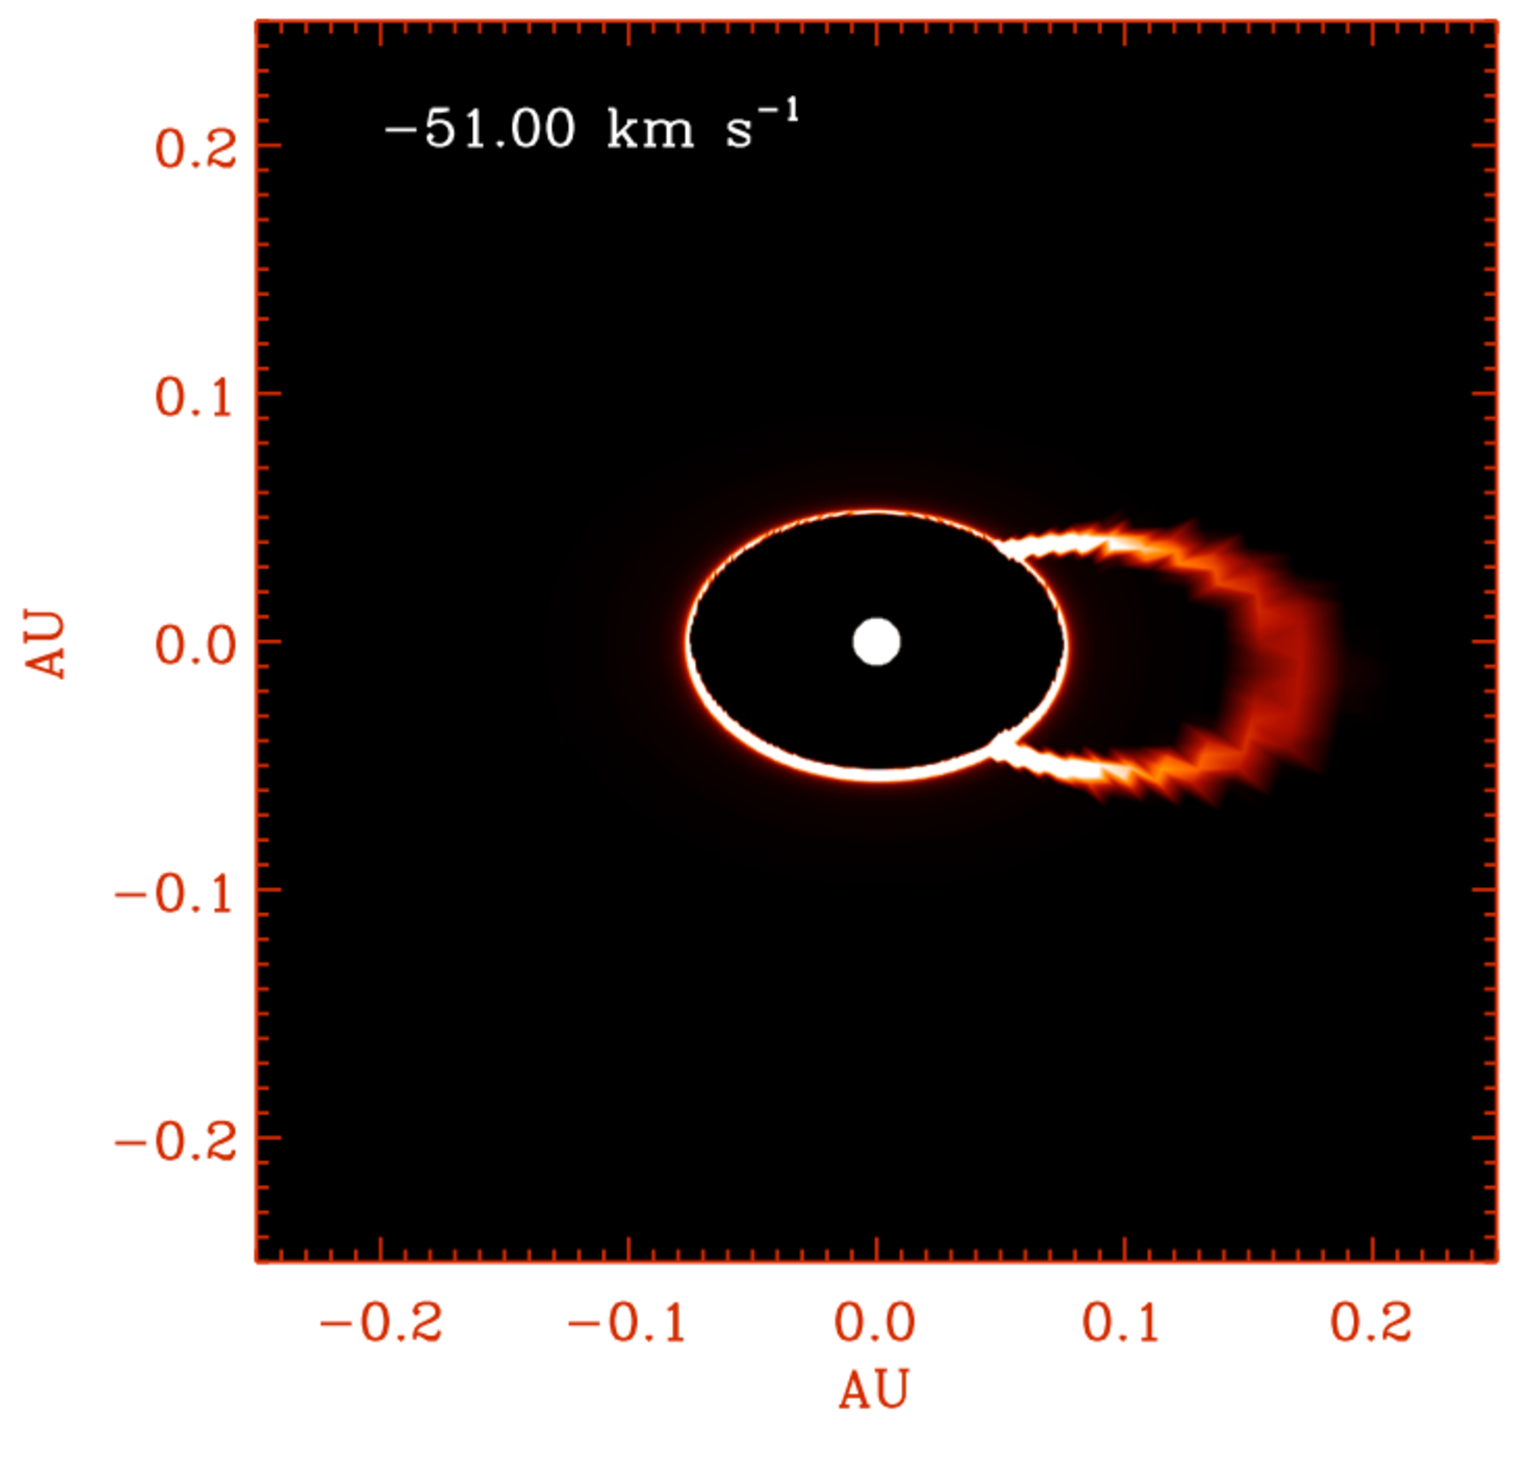
\includegraphics[width=7cm]{imcir_conv_ex1.pdf}
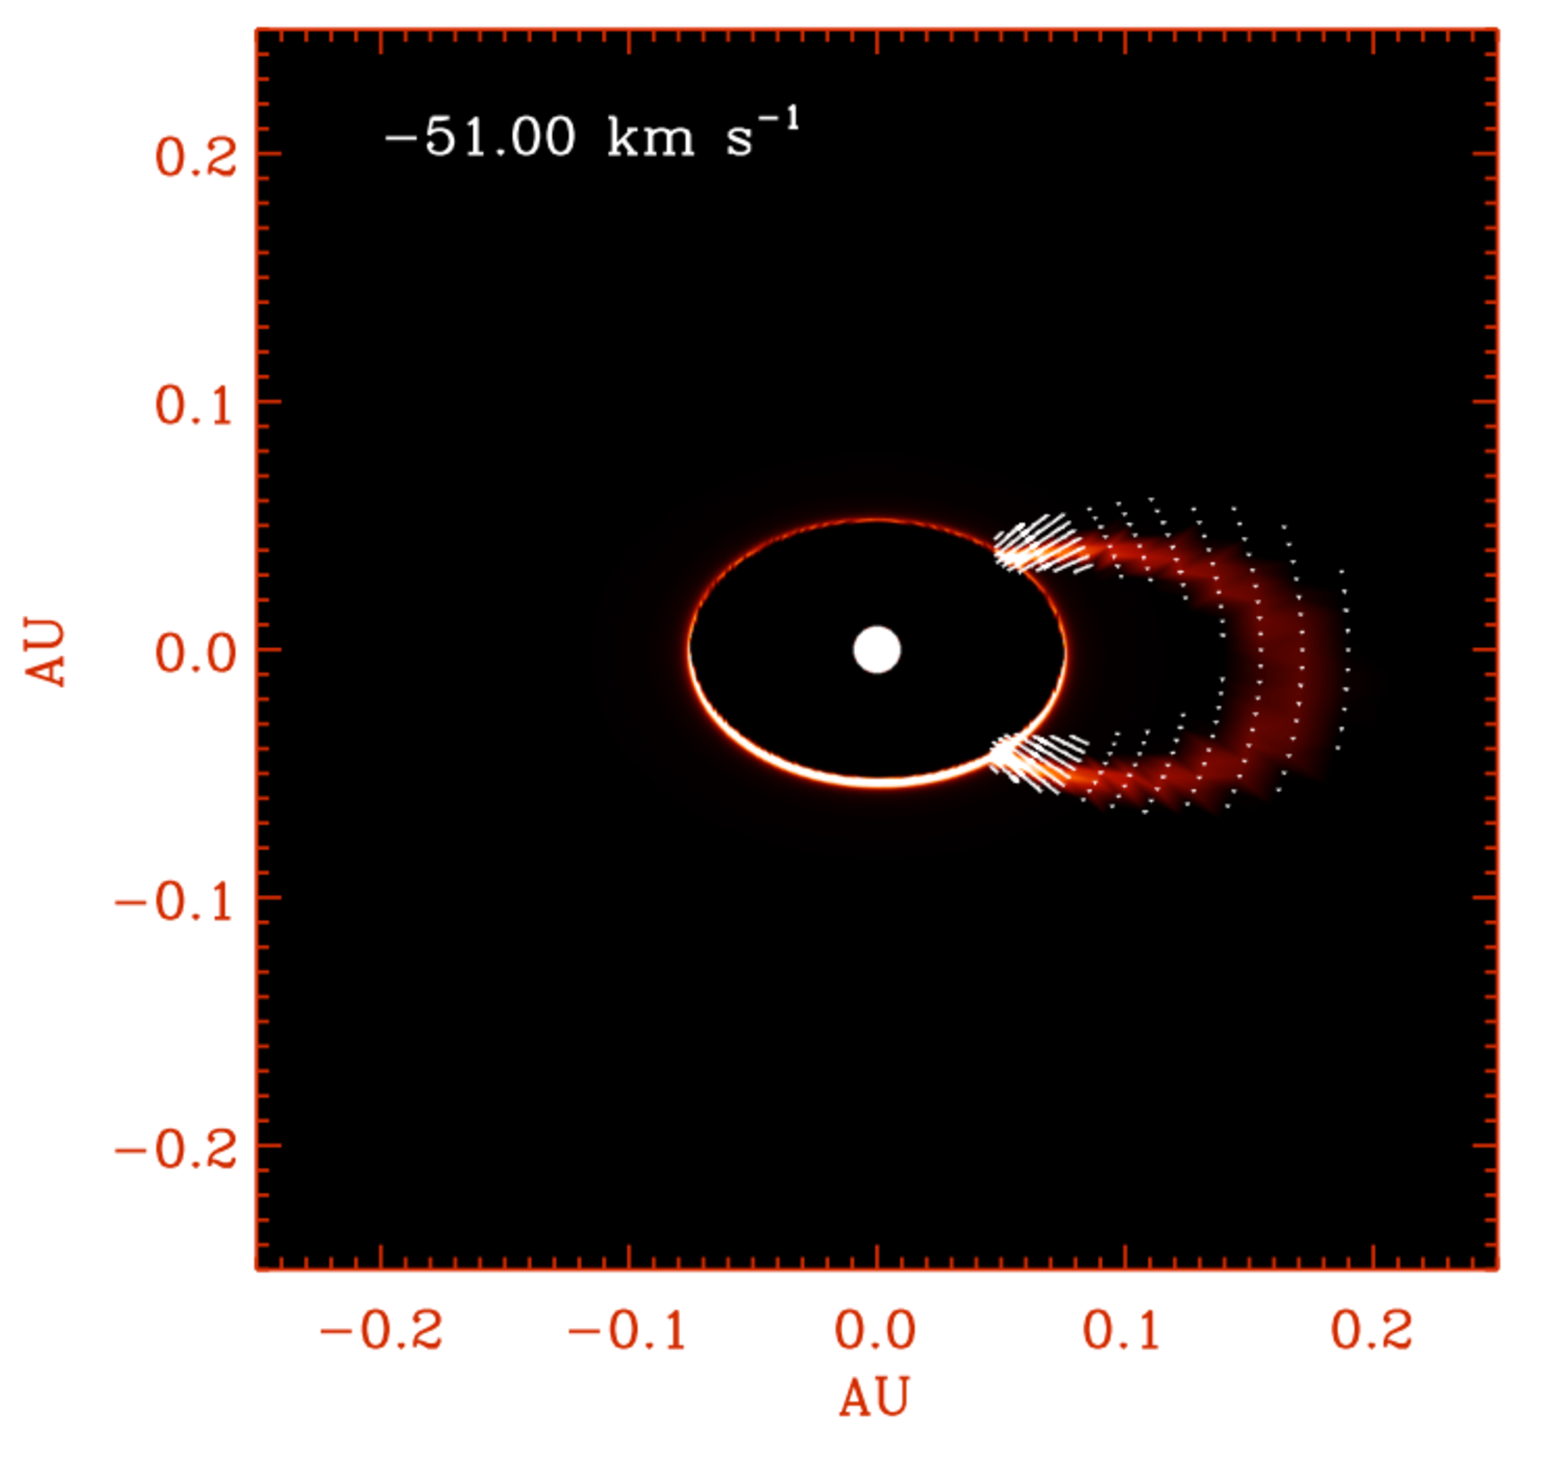
\includegraphics[width=7cm]{imcir_conv_ex2.pdf}
\caption{CO $v=1-0$ P(7) line for the example protoplanetary disk as it appears when generated by RADlite and imaged using {\tt imcir\_conv}.
Left: Intensity map of the -51 km/s channel. Right: Intensity map with the ray configuration overlayed.  }
\label{imcir_ex1}
\end{figure}

The result of this command is shown in the right panel of Figure \ref{imcir_ex1}. Each white dot represents the location of a ray, and consequently the calculation
of a local intensity in units of $\rm erg\,cm^{-2}\,s^{-1}\,Hz^{-1}\,sterad$. The rays must resolve local structure in the intensity map in order for the total flux
to be correct. Plots such as those in Figure \ref{imcir_ex1} allow the user to check for undersampling problems. Note that only the rays that include line emission are
included. This is on purpose, as there is no need for RADLite to recalculate rays that are pure continuum for each velocity channel.

The relevant parameters for sampling of the circular images are {\tt cir\_np}, {\tt b\_per\_r} and {\tt b\_extra}. {\tt cir\_np} is the number of rays in each circle, 
{\tt b\_per\_r} is the number of rays per radial grid point and {\tt b\_extra} is the number of extra ray circles inside the inner radial grid point. For instance, 
the sampling can be improved by increasing {\tt b\_per\_r} from 1 to 3. The result is shown in Figure \ref{imcir_ex3}. 

\begin{figure}
\centering
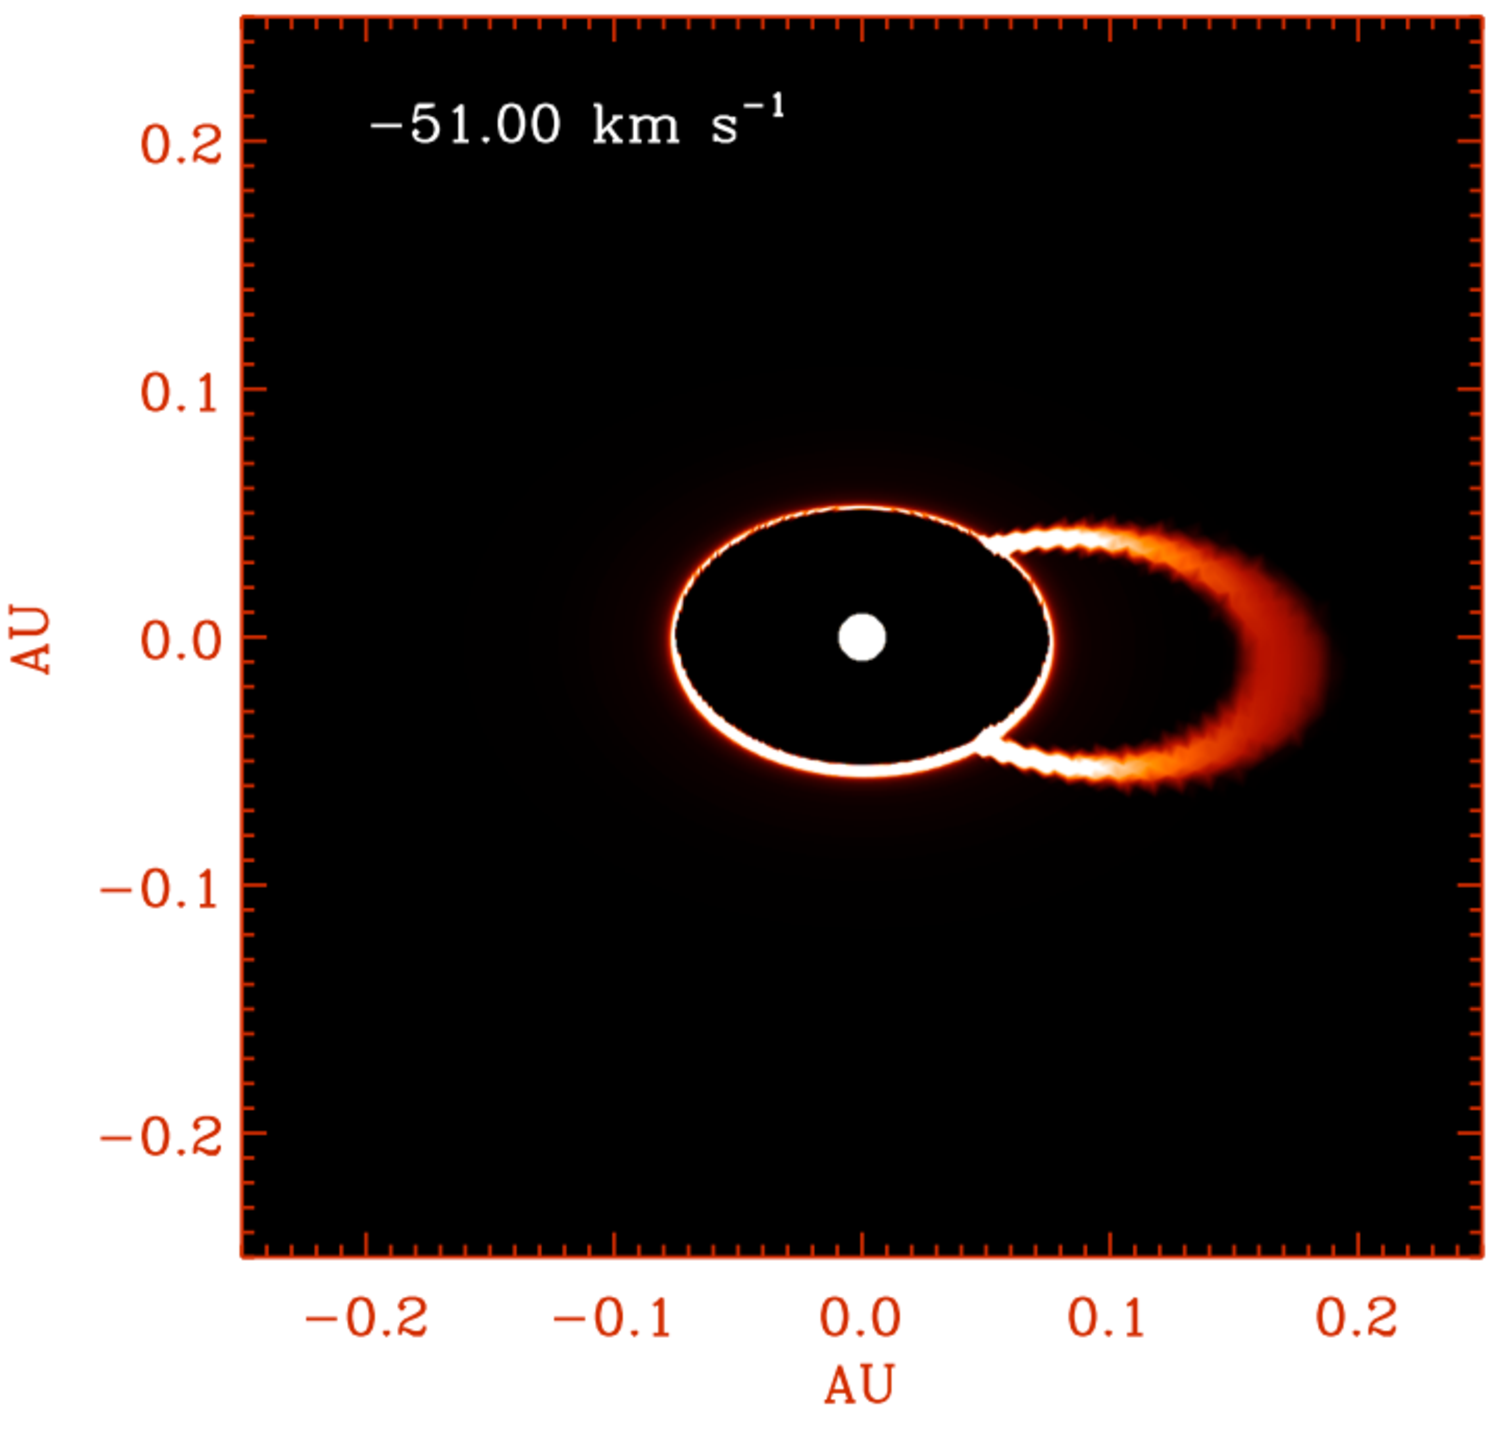
\includegraphics[width=7cm]{imcir_conv_ex3.pdf}
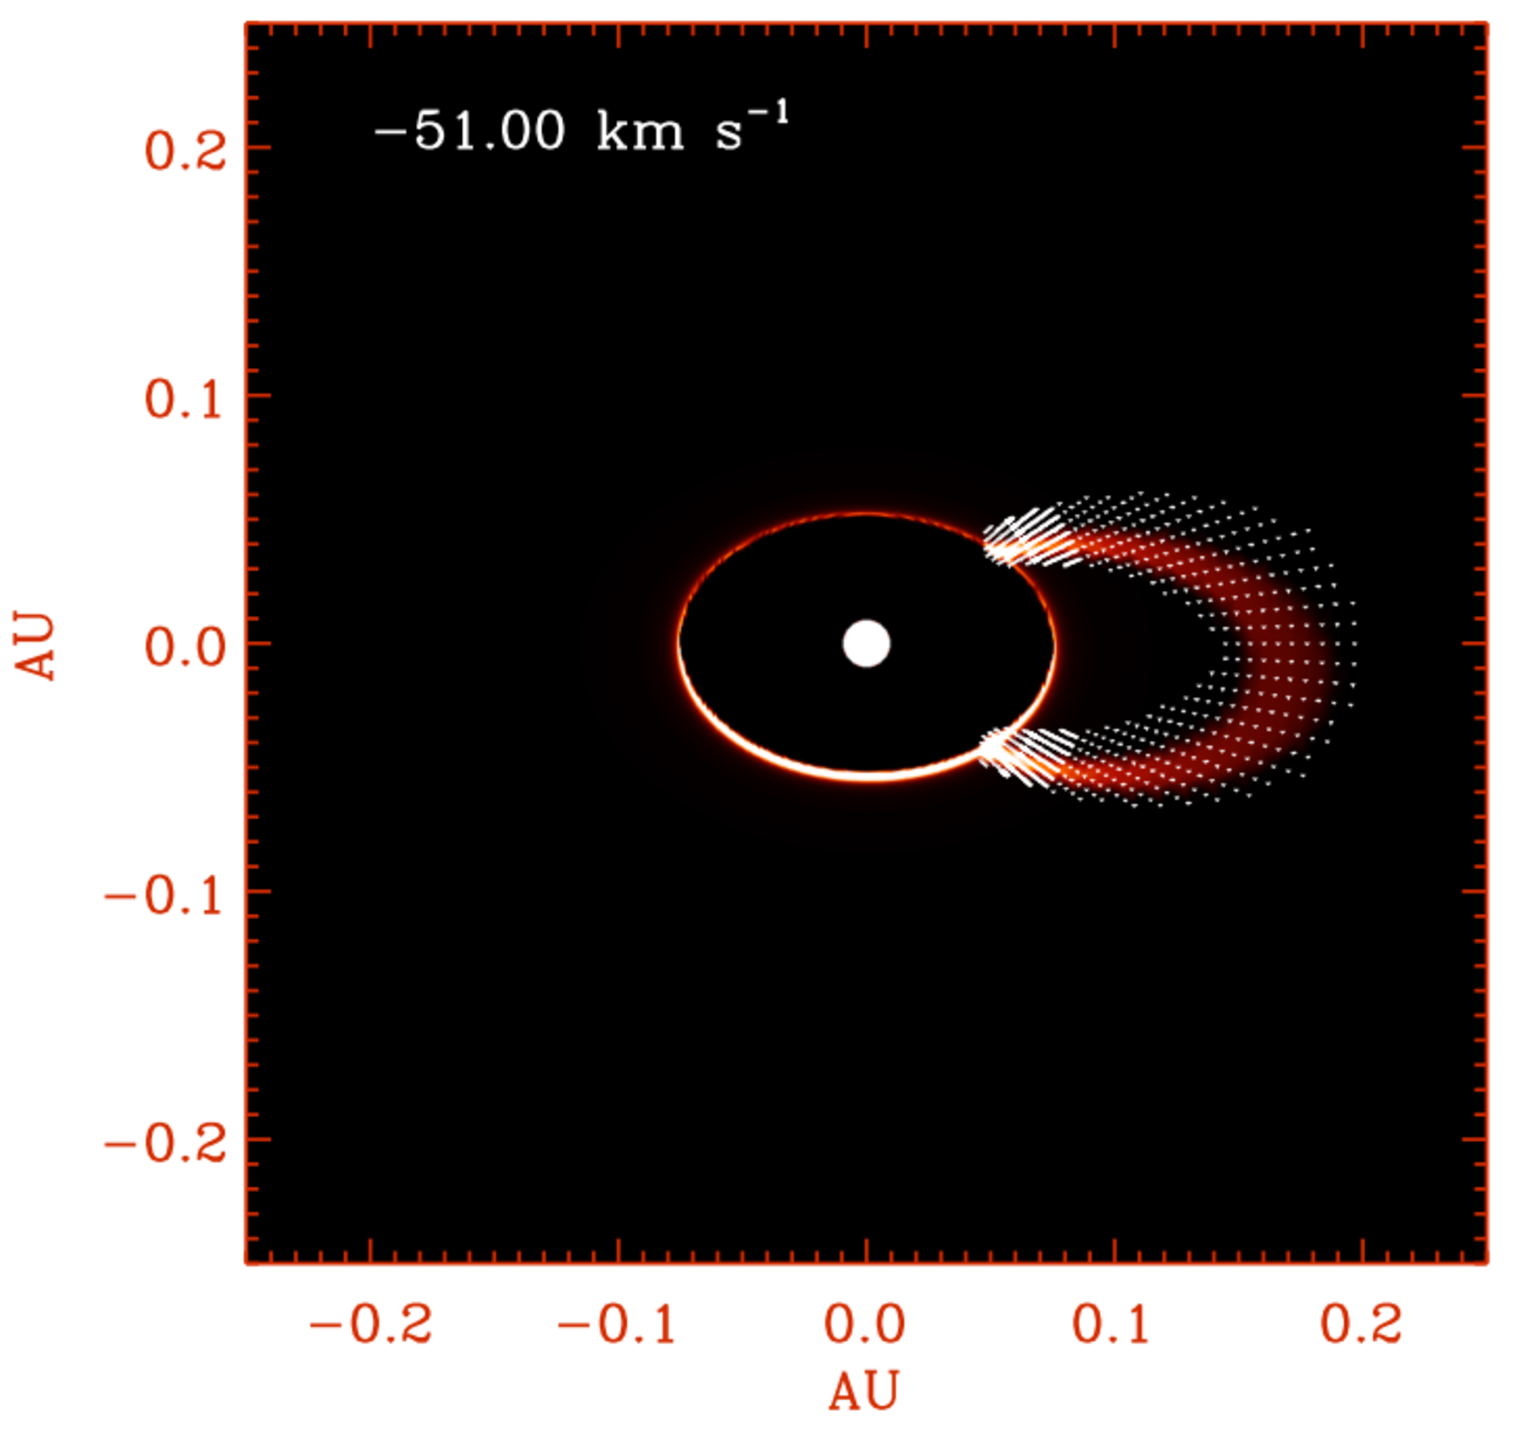
\includegraphics[width=7cm]{imcir_conv_ex4.pdf}
\caption{CO $v=1-0$ P(7) line as shown in Figure \ref{imcir_ex1}, but with a finer radial sampling.  }
\label{imcir_ex3}
\end{figure}

\begin{thebibliography}{}
\small
\bibitem[Dullemond \& Turolla(2000)]{Dullemond00} Dullemond, C.~P., \& Turolla, R.\ 2000, \aap, 360, 1187 
\bibitem[Meijerink et al.(2009)]{Meijerink09} Meijerink, R., 
Pontoppidan, K.~M., Blake, G.~A., Poelman, D.~R., 
\& Dullemond, C.~P.\ 2009, \apj, 704, 1471 
\bibitem[Pontoppidan et al.(2009)]{Pontoppidan09} Pontoppidan, K.~M., 
Meijerink, R., Dullemond, C.~P., \& Blake, G.~A.\ 2009, \apj, 704, 1482 



\end{thebibliography}

\end{document}